\subsection{Multi-View-Coding}\label{subsec:mvc}

\subsubsection{R\"aumliche und Zeitliche Nachbarn eines Rahmens}
\begin{wrapfigure}{r}{0.4\textwidth}
    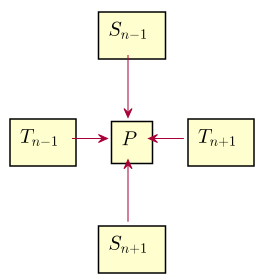
\includegraphics[width=5cm]{../img/prediction}
\end{wrapfigure}

Jeder Rahmen hat drei einzigartige r\"aumliche sowie zeitliche Nachbarn~\cite{paper}.
Diese bestehen aus dem Rahmen der benachbarten Perspektive, dem vorherigen Rahmen der selben Perspektive, sowie
dem vorherigen Rahmen der benachbarten Perspektive.

\noindent\newline Es stellt sich f\"ur uns die Frage, welche der Perspektiven der beste Pr\"adiktor unseres Rahmens ist.
Durch eine statistische Analyse mehrerer Videosequenzen kann diese Frage beantwortet werden.
Hierzu m\"ussen die Kosten des Erstellens eines P-Rahmens zwischen den Nachbarn verglichen werden.
Zwar gibt es starke Variationen zwischen Videosequenzen, im Durchschnitt ist jedoch der direkte zeitliche Nachbar
der beste Pr\"adiktor~\cite{paper}.
Gefolgt wird dieser vom direkten r\"aumlichen Nachbarn.
